\documentclass{article}
\setlength\parindent{24pt}
\usepackage[margin=0.6in]{geometry}
\usepackage{indentfirst}
\usepackage{amsmath}
\usepackage{graphicx}
\usepackage{float}
\usepackage[utf8]{inputenc}
\usepackage{listings}
\usepackage{color}
\usepackage{enumerate}
\usepackage[portuguese]{babel}

\definecolor{dkgreen}{rgb}{0,0.6,0}
\definecolor{gray}{rgb}{0.5,0.5,0.5}
\definecolor{mauve}{rgb}{0.58,0,0.82}

\lstset{frame=tb,
  language=Matlab,
  aboveskip=3mm,
  belowskip=3mm,
  showstringspaces=false,
  columns=flexible,
  basicstyle={\small\ttfamily},
  numbers=none,
  numberstyle=\tiny\color{gray},
  keywordstyle=\color{blue},
  commentstyle=\color{dkgreen},
  stringstyle=\color{mauve},
  breaklines=true,
  breakatwhitespace=true,
  tabsize=4
}

\renewcommand{\baselinestretch}{1.0}

\begin{document}

\title{EA614 - Análise de Sinais \\
\large{EFC5 - Amostragem}}
\author{Rafael Gonçalves (186062)}
\date{\today}

\maketitle

\begin{enumerate}[(a)]
\item
    $y(t)$ - sinal do arquivo 'queen\_I\_want\_it\_all.wav' amostrado em uma taxa Fs = 44,1 kHz.

\item
    Gráfico do espectro de frequência do sinal $y(t)$:
    \begin{figure}[H]
    \centering
    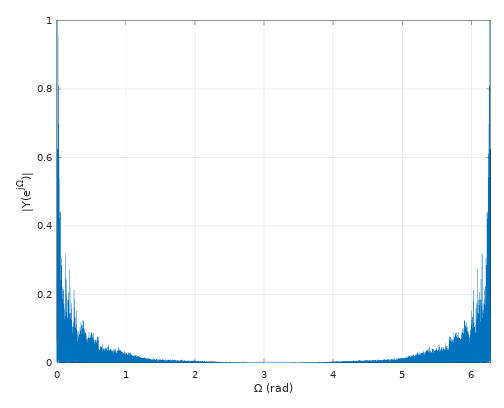
\includegraphics[width=0.3\textwidth]{images/spectre.png}
        \caption{Espectro de frequência $Y(j\Omega)$ em função de $\Omega$}
    \end{figure}

        Há a predominância do sinal nas "bordas" do gráfico (perto de $\Omega = 0 \text{ e } \Omega = 2\pi$, ou seja, baixas frequências). Nas frequências mais altas (intervalo aproximadamente igual a 1 $< \Omega <$ 5) o sinal é praticamente nulo. 

\item
    $y_{dec}(t)$ - sinal do arquivo 'queen\_I\_want\_it\_all.wav' amostrado em uma taxa Fs\_dec = Fs/6 = 7,35 kHz.

    Gráfico do espectro de frequência do sinal $y_{dec}(t)$:
    \begin{figure}[H]
    \centering
    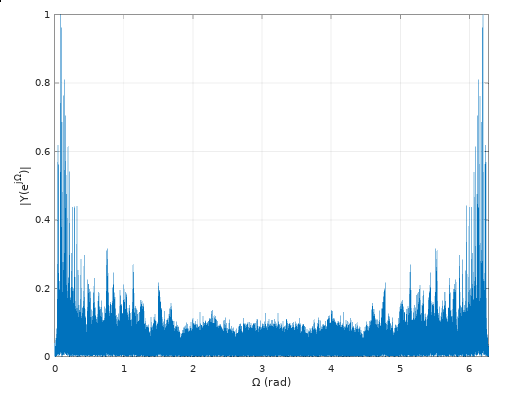
\includegraphics[width=0.3\textwidth]{images/spectre_dec.png}
        \caption{Espectro de frequência $Y_{dec}(j\Omega)$ em função de $\Omega$}
    \end{figure}

        Embora o perfil do espectro seja similar ao do sinal original, têm-se a impressão de que foi adicionado um ruído em todas as frequências (valor de $Y_{dec}(j\Omega)$ é maior que 0.1 em para praticamente todos os valores de $\Omega$, por exemplo). Há uma distorção bastante perceptível para as frequências altas que eram praticamente nulas no espectro original. Esse ruído também é percebido pois há uma consistencia menor do sinal, enquanto que a curva original era mais bem definida, nesta há uma ocorrência maior de vales e picos durante todo o espectro (em especial nas frequências menores).

\break\vfill

\item
    O sinal subamostrado tem um som "abafado" quando comparado com o original. Também parece haver uma diminuição dos graves (baixas frequências) em relação aos agudos (altas frequências). Há uma dificuldade maior em distinguir os sons (instrumentos, voz) por conta destes aparecerem com um chiado. 

\item
    Gráficos das respostas em frequência $h(t)$:

    \begin{figure}[H]
    \centering
    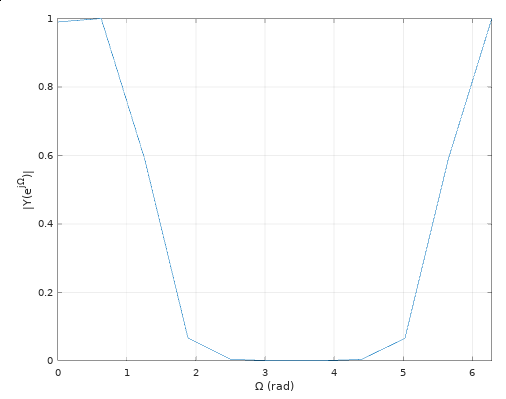
\includegraphics[width=0.3\textwidth]{images/h1.png}
        \caption{Filtro Kaiser $\Omega_p = 0.45$ e $\Omega_r = 2$}
    \end{figure}

    \begin{figure}[H]
    \centering
    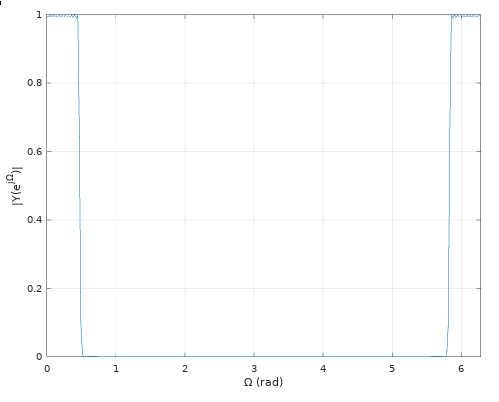
\includegraphics[width=0.3\textwidth]{images/h2.png}
        \caption{Filtro Kaiser $\Omega_p = 0.45$ e $\Omega_r = 0.5$}
    \end{figure}

    \begin{figure}[H]
    \centering
    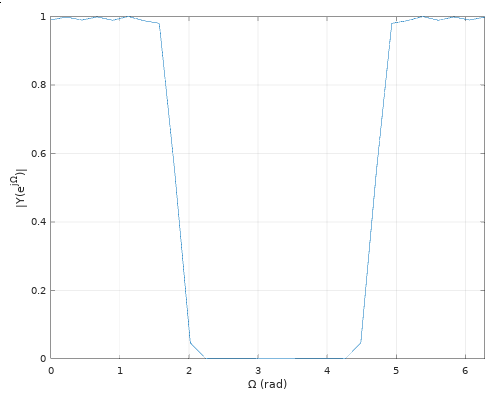
\includegraphics[width=0.3\textwidth]{images/h3.png}
        \caption{Filtro Kaiser $\Omega_p = 1.5$ e $\Omega_r = 2$}
    \end{figure}

        Os 3 filtros são filtros passa-baixa em que as frequências entre $\Omega = 0$ e $\Omega = \Omega_p$ são próximas de um enquanto que as frequências a partir de $\Omega = \Omega_r$ até $\Omega = \pi$ são próximas de zero. O filtro é simétrico centrado em $\pi$, pois o espectro de um sinal discreto é periódico com período $2\pi$ (baixas frequências nas extremidades e altas frequências próximas a $\Omega = \pi$). Quanto menores os valores de $\Omega_p$ e $\Omega_r$, uma faixa maior de frequências altas é rejeitada. Quanto mais próximos os valores de $\Omega_p$ e $\Omega_r$, mais rápida é a transição do filtro entre passagem e rejeição, no caso oposto, mais suave é a transição entre passagem e rejeição.

\break\vfill

\item
    Gráfico da respostas em frequência de $h(t)*y(t)$:

    \begin{figure}[H]
    \centering
    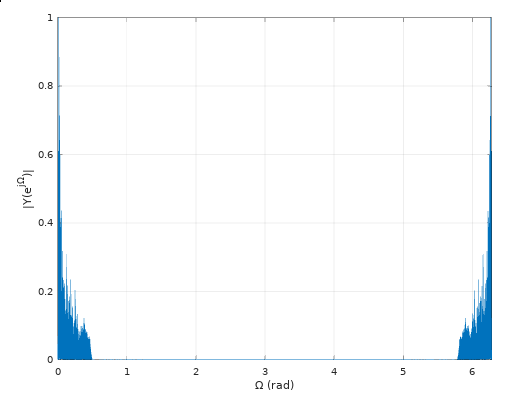
\includegraphics[width=0.5\textwidth]{images/conv_h.png}
        \caption{$y(t)$ aplicado o filtro Kaiser $\Omega_p = 0.45$ e $\Omega_r = 0.5$}
    \end{figure}

    O espectro resultante é praticamente o sinal original com as frequências entre $\Omega = 0.5 \text{ e } \Omega = 2\pi - 0.5$ removido.
    Após aplicado o filtro, há uma redução dos agudos e o som parece mais "abafado" se comparado ao sinal original.

\item
    Gráfico da respostas em frequência de $h(t)*y(t)$ com M = 6:

    \begin{figure}[H]
    \centering
    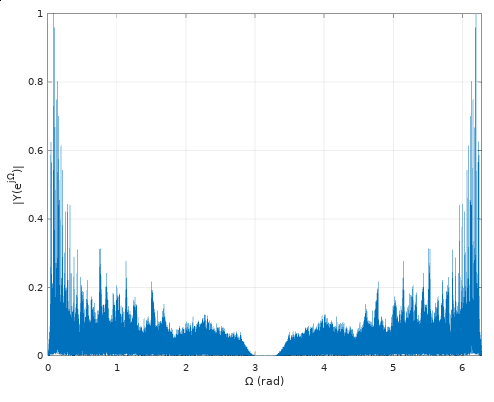
\includegraphics[width=0.5\textwidth]{images/resamp_after_filter.png}
        \caption{$y(t)$ amostrado com M=6 após ter sido aplicado o filtro Kaiser $\Omega_p = 0.45$ e $\Omega_r = 0.5$}
    \end{figure}

    O espectro ainda distorceu o sinal original, aumentando a quantidade de picos e vales, porém desta vez não contém frequências muito altas ($\Omega \text{ muito próximo de } \pi$). Há esse ruído que continua bastante perceptível sobretudo para as baixas frequências.

    O som continua "abafado", porém houve redução do chiado (som parece mais "limpo") se comparado ao sinal subamostrado sem o uso do filtro.Também comparando esses sinais, nesse com o filtro, fica mais fácil identificar os sons da voz e dos instrumentos.

\end{enumerate}
\end{document}
